\documentclass{report}
\usepackage{algorithm2e}
\usepackage{tikz}
\usetikzlibrary{arrows, snakes, shapes, positioning, shadows, trees}
\title{User and Reference Manual of BinCAT}
\author{Sarah Zennou\\sarah.zennou@airbus.com}
\begin{document}
\maketitle
\tableofcontents
\chapter{Installation}

\section{Dependencies}
\chapter{Documentation}
can be found in html and latex format for both python and ocaml in doc/generated/[python|ocaml]/[html|latex]

\chapter{Architecture}
{
\tiny
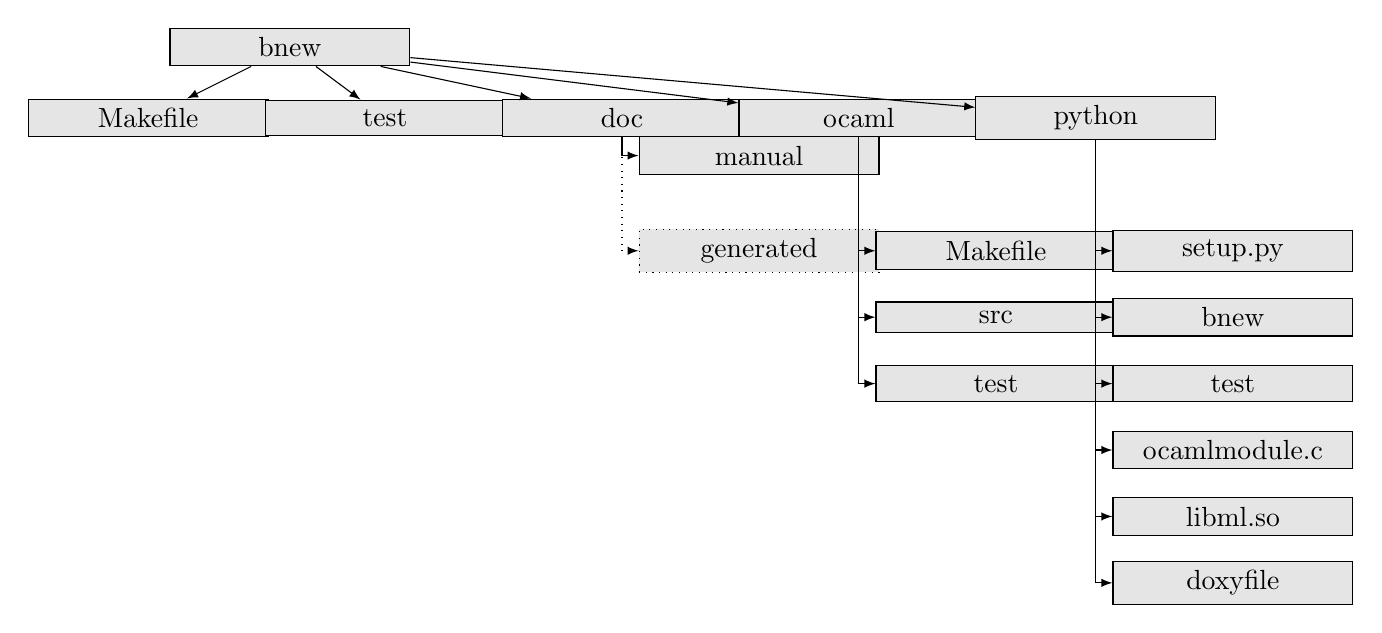
\begin{tikzpicture}
[scale=0.6,
  every node/.style={draw, text width=8em, thin, align=center, fill=gray!20},
  edge from parent/.style={->,draw},
  grandchild/.style={grow=down,xshift=1em,anchor=west,
    edge from parent path={(\tikzparentnode.south) |- (\tikzchildnode.west)}},
  >=latex]

\node (root) {bnew}
 child{
    node(makefile) {Makefile}
  }
  child[xshift=10em]{
    node(test) {test}
  }
  child[xshift=20em] {
    node (doc) {doc}
    child[grandchild, yshift=2em] {
      node (manual) {manual}
    }
    child[grandchild, level distance=8em, dotted] {
      node (generated) {generated}
    }
  }
  child[xshift=30em] {
    node (ocaml) {ocaml}
    child[grandchild, level distance=8em] {
      node (mlmake) {Makefile}
    }
      child[grandchild, level distance =12em] {
      node (mlsrc) {src}
    }
    child[grandchild, level distance =16em] {
      node (mltest) {test}
    }
  }
child[xshift=40em] {
    node (python) {python}
child[grandchild, level distance=8em] {
      node (setup) {setup.py}
    }
      child[grandchild, level distance =12em] {
      node (pysrc) {bnew}
    }
    child[grandchild, level distance =16em] {
      node (pytest) {test}
    }
    child[grandchild, level distance =28em] {
      node (doxyfile) {doxyfile}
    }
child[grandchild, level distance =24em] {
      node (mlc) {libml.so}
    }
child[grandchild, level distance =20em] {
      node (mlc) {ocamlmodule.c}
    }
  }
;


\end{tikzpicture}
}

\chapter{Big Picture}

\chapter{Internals of the Control Flow Graph}
Its signature is \verb|src/data-struct/cfg.mli|
Its implementation is in \verb|src/fixpoint/fixpoint.ml|\footnote{cannot be
separated from the fixpoint engine
as decoding and analyzing are interleaved and both depend on the type
of Data analyzed. Failed to solve of mutual functor dependencies gives
rise to this solution}

\section{nodes}
A node represents a \emph{state machine} at a given \emph{program counter value} 
in a given \emph{context}.
\subsection{State machine}
A state machine is a map 
\begin{itemize}
\item from register to abstract values
\item from memory addresses to abstract values
\item from stack offsets to abstract values

\end{itemize}
\subsection{Program Counter}
\subsection{Context}
\section{Edges}
\chapter{Abstract Values}
\section{Current Domains}
\subsection{ptr}
concrete ptr
\subsection{tainting}
3-valued vector: tainted/untainted/top

\section{Reduced Product}
no reduction

\chapter{Fixpoint Computation}
Implementation is in \verb|src/fixpoint/interpreter.ml|

A control flow automation \emph{A} is a data structure made of the following fields:
\begin{itemize}
\item cfg: the already built control flow graph;
\item state: the current abstract state machine. It is composed of 
  \begin{itemize}
  \item store: the current abstract store  (see
  section ...);
\item pc: the current program counter value
\item ctx: the dcoding context (operand size, address size)
\end{itemize}
\end{itemize}

\begin{figure}
\begin{algorithm}[H]
\SetKwFunction{Decode}{Decode}
\SetKwFunction{ProcessStmt}{ProcessStmt}
\SetKwFunction{Fold}{Fold}
\SetKwFunction{MakeNode}{makeNode}

\KwData{c: code string}
\KwData{A: a control flow automaton}
\KwResult{the updated Control Flow Automaton}
\BlankLine
\emph{waiting $\leftarrow$ \{(A.state})\}\;
\While{waiting is not empty}{
  \emph{let $s$ be a state in waiting}\;
  \emph{remove $s$ from waiting}\;
  \emph{l $\leftarrow$ Decode(c, s.pc, s.ctx)}\;
  \For{$(i, pc', ctx') \in l$}{
    store' $\leftarrow Fold (\lambda~s. ProcessStmt(i, s), i, s.store)$\;
    $n \leftarrow$ MakeState(store', pc', ctx')\;
  \If{$n$ is not in A.cfg}{
    \emph{add $n$ to waiting\;}
    \emph{add the node n to ctx.cfg\;}
    \emph{add an edge $s \to n$ in A.cfg\;}
    }
}
}
\Return{ctx}
\end{algorithm}
\caption{The Fixpoint Algorithm}
\end{figure}
Remarks:
  \begin{itemize}
\item the decoding context may change because of the presence of a
  prefix in the x86 instruction to decode (see line xx (for loop))
\item functions Decode, ProcessStmt (see figure \ref{algo:processStmt}), Fold, etc.
\item the data structure of the code string has to maintain the
  address of its first element (needed in the function Decode)
\item decode returns a list of IL statement lists
\item in particular processStmt is in charge of checking whether a
  widening is needed to ensure termination of the fixpoint computation
  \end{itemize}

\begin{figure}
\begin{algorithm}[H]
\end{algorithm}
\caption{The ProcessStmt Algorithm}
\label{algo:processStmt}
\end{figure}
\chapter{User Interactions}
\section{Data Tainting Inputs}
\section{Breakpoints}
\section{Backtracking}

\chapter{Implementation remarks}

From Kinder:
``The virtual memory available to a process is organized as one large,
continous array. The stack, the heap and global variables all share
this address space. The runtime environment initializes the stack and
heap locations to reasonable values such that they do not interfere,
and it uses buffer pages between these logical memory regions to
detect overflows.

Correct implementations of malloc (and its kernel-level equivalents
available to drivers) guarantee thatr allocated memory blocks in the
heap do not overlap.``

=> on peut utiliser des regions abstraites pour Global, Stack et Heap.

Actuellement, les sélecteurs de segments peuvent contenir des valeurs
qui ne correspondent à aucun descripteur de segment.

Special effort to be as generic as possible.
Modules and functors that are achitecture dependent are:
\begin{itemize}
\item decoder.ml (x86 on 32 bits)
\item parser.mly
\item lexer.mll
\item abi.ml x86 because of need to know mode protected/real and
  presence or not of segment selectors in the address generation from
  a string
\item one line in main.ml that generates the address of the entry
  point from the configuration file (and hence from !Config.cs)
\end{itemize}


\chapter{Optimisations}
dot not decode twice if the context is the same (including the
internal state of the decoder)
\chapter{known bugs}
printed line of a bug in parsing is wrong
\chapter{Quality improvements}
add .mli
\chapter{Glossary}
\begin{itemize}
\item control flow automaton
\item abstract state
\item decoding context
\item program counter
\end{itemize}


\end{document}
